The HAT-P-37 system is present in 11 different sectors of TESS with a cadence of 120.0 s. Previously timing data from only one sector (59) has been published. \cite{wangLongtermVariationsOrbital2024} Upon investigation, 9 out of the 10 unpublished sector lightcurves produced by the TESS-SPOC pipeline in the lightkurve package show significant contamination of the HAT-P-37 flux. Using the MAST database(?), we were able to determine that the main source of this contamination was a nearby variable star, ZTFJ185715.34+511631.4, which is a W Ursae Majoris (EW)-type Eclipsing binary, as characterized by Chen et. al.\citep{chenZwickyTransientFacility2020}. For simplicity, we will refer to this star as "EB" from here on. 

Using the orbital period from Chen et. al. and the tools in the lightkurve package, we have been able to separate the transit light curves for HAT-P-37 b from the variability of the EB. Figure \ref{fig:EB_folded} depicts all 11 sector's PDCSAP flux phase folded to the parameters of the EB as published previously. This figure shows that the amount of contamination varies from sector to sector, leading to a sector specific approach being necessary to remove the contamination and fit the transit light curves of HAT-P-37 b.

\begin{figure}
    \centering
    \includegraphics[width=0.9\linewidth]{figures/all_sectors_folded_EB_period.png}
    \caption{TESS sectors phase folded on the period of the EB. Each sector is affected by a different amount of contamination and as such each sector will need to be detrended separately.}
    \label{fig:EB_folded}
\end{figure}

TESS Sector used in this study: 

\begin{itemize}
    \item 26 - Average fraction of flux of the target star:  76.932538 \%
    \item 40 - Average fraction of flux of the target star:  65.78933599999999 \%
    \item 41 - Average fraction of flux of the target star:  66.98885 \%
    \item 53 - Average fraction of flux of the target star:  60.779458 \%
    \item 54 - Average fraction of flux of the target star:  64.582843 \%
    \item 55 - Average fraction of flux of the target star:  74.128646 \%
    \item 59 - large dip approx. 12 day period, masked in PDCSAP flux, but probably need to look into what it is - Average fraction of flux of the target star:  58.385509 \%
    \item 74 - no contamination with EB - fit fine as it - Average fraction of flux of the target star:  59.20288 \%
    \item 75 - no contamination with EB - fit fine as it - Average fraction of flux of the target star:  59.999548999999995 \%
    \item 80 - Average fraction of flux of the target star:  65.208763 \%
    \item 82 - Average fraction of flux of the target star:  66.821003 \%
\end{itemize}

\begin{figure}
    \centering
    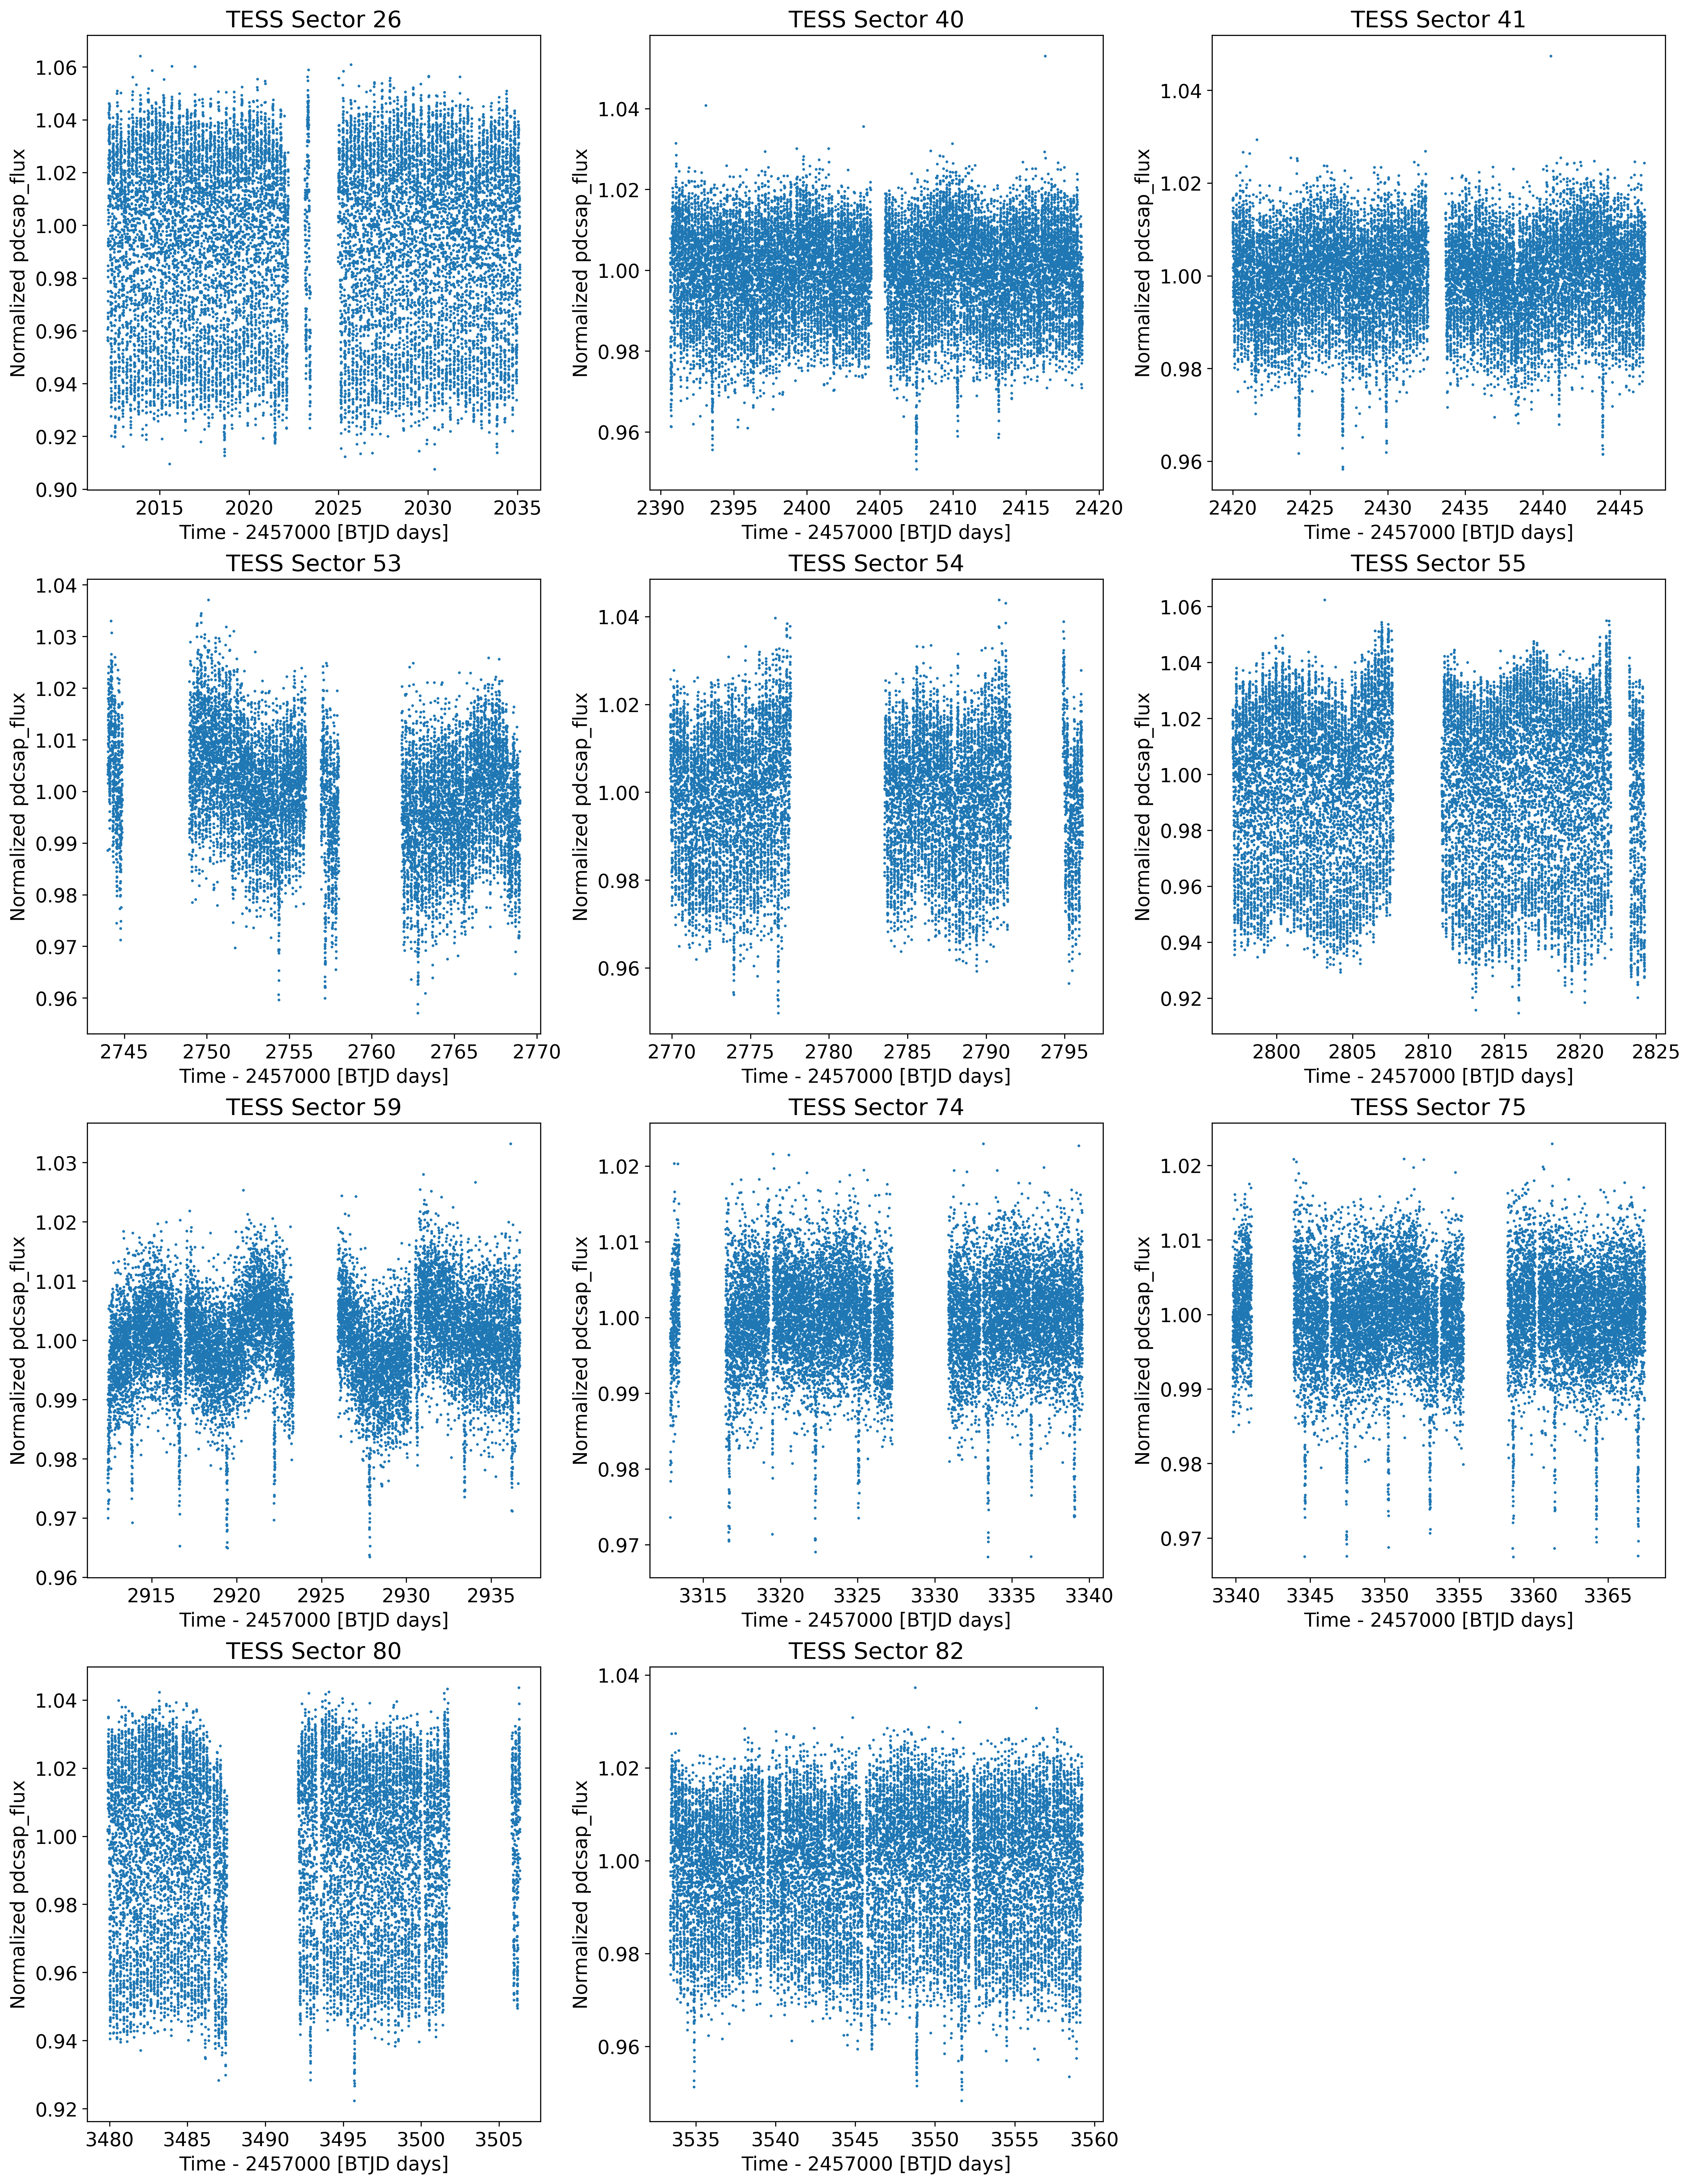
\includegraphics[width=\linewidth]{code/figures/allSectors_sigma5_PDCSAPflux_lc.png}
    \caption{PDCSAP flux for each sector of Tess data}
    \label{fig:enter-label}
\end{figure}

TESS Sectors 74 and 75 did not show significant contamination and were able to be fit using the analysis as described in Adams et. al. \citep{doomed_worlds1}. We also exclude Sector 59 from this analysis and use the mid-times as reported in Wang et. al. 

\begin{figure}
    \centering
    \includegraphics[width=\linewidth]{figures/wellbehaved_sectors_LS_periodogram.png}
    \caption{Lomb-Scargle Periodogram of the TESS sectors used in this study. Each sector returns a period at maximum power approximately one-half of the expected period of that of the EB.}
    \label{fig:LS}
\end{figure}

For these contaminated sectors, ...